\section{Эксперимент}
Все ниже перечисленные реакции относятся к типу 
реакций замещения. В ходе данных реакций к металлы 
$Br, Na, K$ замещаются металлами более реакционным 
металлами $Ag, Pl$. 
\begin{equation} 
    NaCl|KBr|KI + AgNO_3 \xrightarrow{}   AgCl|Br|I\downarrow + NaNO_3
\end{equation} 
\begin{equation} 
    2NaCl|2KBr|2KI + Pb(NO_3)_2 \xrightarrow{}  PbCl_2|Br_2|I_2\downarrow  + 2 KNO_3
\end{equation} 
В образовашейся смеси соли $PbCl_2|Br_2|I_2 \land AgCl|Br|I$
являются нерастворимыми, поэтому они выпадут 
в виде осадка.

\begin{center}
\begin{tabular}{l||l||l}
    Compound & Color & Transparency \\ \hline \hline
    $AgCl$ & Светло серый $\to$ белоснежный & Непрозрачный \\
    $AgBr$ & Бело-желтовытый & Непрозрачный\\
    $AgI$ & Желтый & Непрозрачный\\
    $PbCl_2$ & Белый & Непрозрачный \\
    $PbBr_2$ & Бледно-желтый & Непрозрачный \\
    $PbI_2$ & Желтый & Непрозрачный \\
\end{tabular}
\end{center}

\begin{figure}[h]
    \centering
    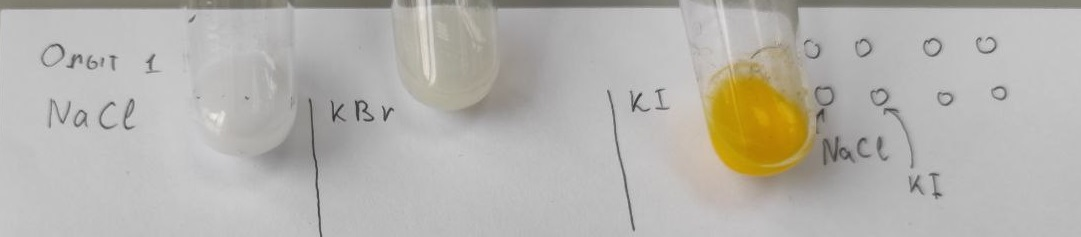
\includegraphics[width=1\linewidth]{Ex_1/1.jpg}
     \caption{$AgCl, AgI, AgBr$}
    \label{ex_1_1}
\end{figure}

\begin{figure}[h]
    \centering
    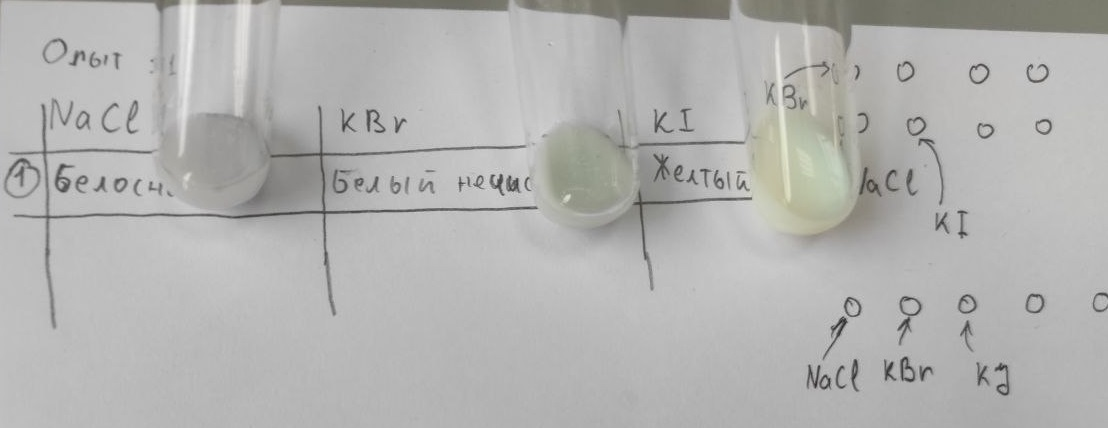
\includegraphics[width=1\linewidth]{Ex_1/2.jpg}
     \caption{$PbCl_2, PbBr_2, PbI_2$}
    \label{ex_1_2}
\end{figure}